
\section{Evaluation}
\label{sec:eval}
\vspace{-0.2cm}
%		\par Figure showing nvprof metrics for all 10 application kernels and the closest match from the microbenchmark. Figure showing similarity of microbench and kernel corun 2D spaces for one kernel pair. Use these figures to argue that we have a good way to get pre-generated data which mirrors the contention properties of the application kernels.
%		\par Show that the 2D spaces are off by nearly a constant in the QoS ratio, possibly another figure to show how close a constant factor adjustment gets them to matching

%\begin{figure}
%	\centering
%	\caption{Co-Running Windows Explainer}
%	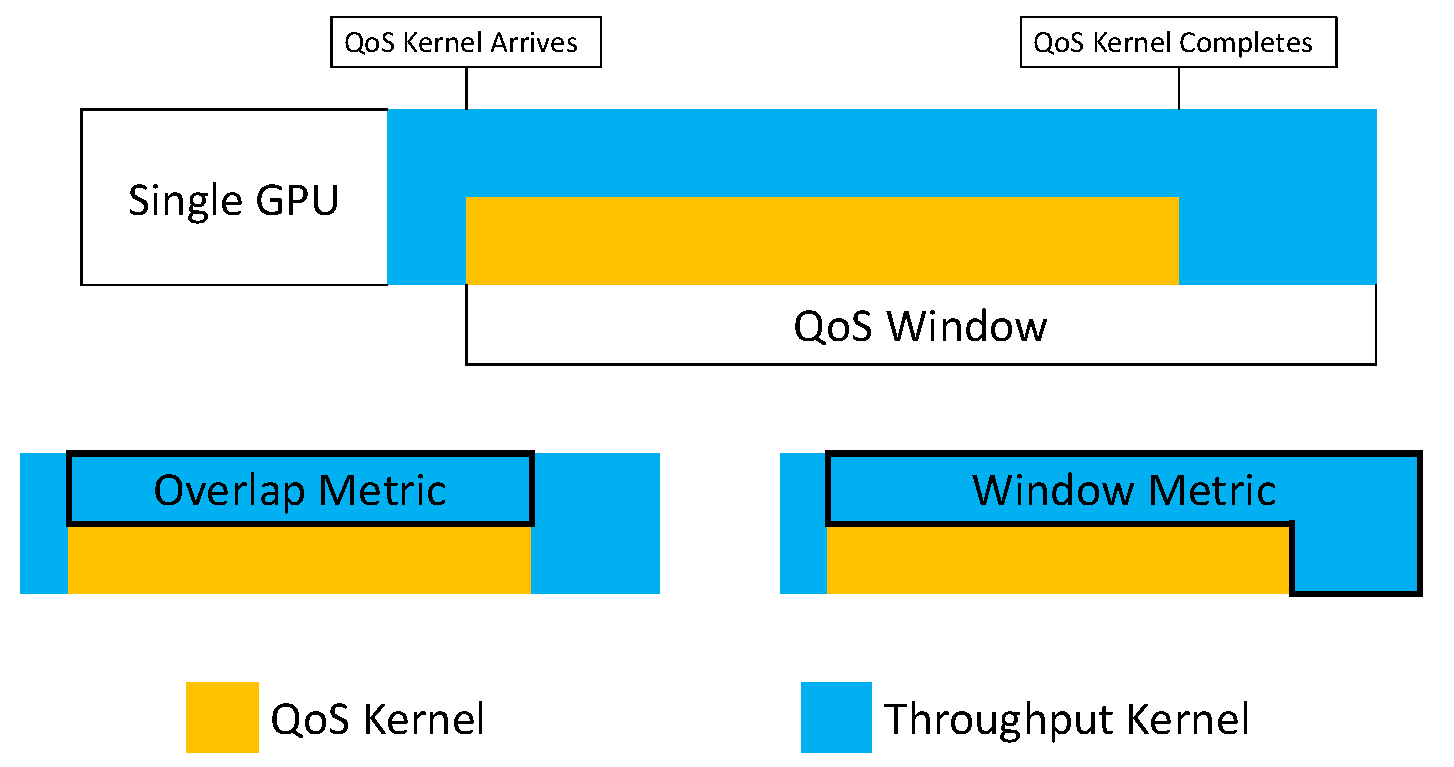
\includegraphics[width=8cm]{figures/corun_windows_cropped.pdf}
%	%\vspace{-1cm}
%	\label{fig:corun-windows}
%\end{figure}

%Short summary of this section
%\par This section presents the experimental results for the performance of the approaches presented in this paper.

\subsection{Experimental Setup}
\begin{figure*}
        \vspace{-1cm}
        \centering
        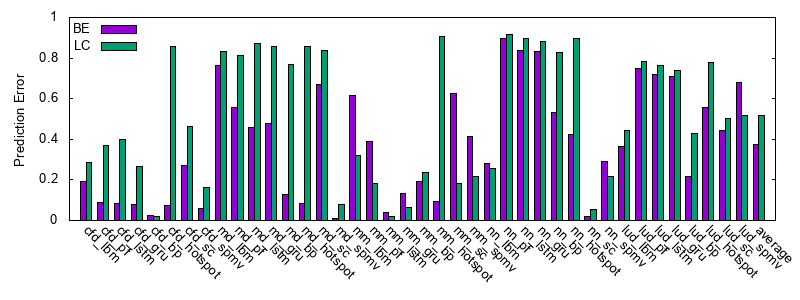
\includegraphics[width=\textwidth,height=2.5cm]{figures/new_error_res.png}
        %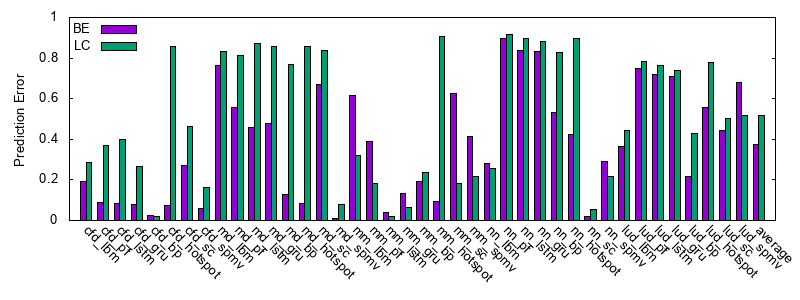
\includegraphics[width=\textwidth]{figures/new_error_res.png}
        \caption{Performance estimation error evaluation.}
        \label{fig:error}
        \vspace{-.5cm}
\end{figure*}
%\begin{table}
%\scriptsize
%\vspace{-0.5cm}
%\centering
%    \caption{System Setup}
%    \begin{tabular}{ c | c }
%        \hline
%        CPU & 2S Intel Xeon E7-4830 v3 @ 2.1 GHz \\
%        GPU & NVIDIA TITAN V100 w/ 12GB GDDR5X \\
%        \hline
%        OS & Ubuntu 16.04 x64 with kernel 4.4.0-128 \\
%        CUDA & Driver 418.56 CUDA SDK 10.1 \\
%        \hline
%    \end{tabular}
%    \label{tbl:system}
    %\vspace{-.5cm}
%\end{table}
\par We evaluate FLARE using an NVIDIA TITAN V GPU with 12GB onboard memory hosted by a server with an Intel Xeon E3-1286 v3 CPU and 32GB main memory. The system runs Ubuntu 16.04 with kernel version 4.4.0-141, NVIDIA driver 410.48, and CUDA 10.0.
%The table \ref{tbl:apps} shows
We focus our evaluation on eleven benchmarks and two real-world applications. The benchmarks are from three popular benchmark suites: Rodinia~\cite{Rodinia}, SHOC~\cite{SHOC},
and NVIDIA's CUDA SDK. Two real applications,
TC~\cite{text} and CN~\cite{Sutskever:ICML11}, represent deep learning inference workloads. TC uses an LSTM~\cite{LSTM} model to classify documents and 
CN uses a GRU~\cite{GRU} model to predict the likely next character given an input string. Both of these inference applications heavily utilize the GPU, and are classified as LC applications. We also evaluate SPMV (SHOC), SC, PF, HOTSPOT, LBM and BP (Rodinia) as LC applications and MD (SHOC), MM (CUDA SDK), NN, LUD and CFD (Rodinia) as BE applications. Only the BE applications require adaptation to yield resources, while the LC applications can run unmodified.
%The table also identifies which applications are classified as BE and LC applications
%shown by the ``Role'' column. Every co-run pair presented in this section is composed of one BE application and one LC application.
%The goal is to maximize the throughput achieved while still completing the QoS kernel within a deadline. Unless otherwise noted, that deadline is assumed to be 2 times the duration the kernel takes when running alone on the GPU, also referred to as a QoS ratio of 2.
%\begin{table}[ht]
%\centering
%\scriptsize
%\begin{minipage}
%\centering
%    \caption{Benchmarks}
%    \begin{tabular}{ | l | c | c | c |}
%        \hline
%        {\bf App.} & {\bf Source} & {\bf Description} & {\bf Role} \\ \hline \hline
%        CFD & Rodinia & finite volume solver & BE \\ \hline
%        MD  & SHOC & molecular dynamics & BE \\ \hline
%        MM & CUDA SDK & dense matrix multiplication & BE\\ \hline
%        NN  & Rodinia & nearest neighbor & BE \\ \hline
%        %PL & Rodinia & bayesian framework & BE \\ \hline
%        BP & Rodinia & backpropagation& LC \\ \hline
%        LBM & Rodinia & fluid dynamics & LC\\ \hline
%        HOTSPOT & Rodinia & thermo dynamics & LC \\ \hline
%        PF  & Rodinia & dynamic programming & LC \\ \hline
%        SC  & Rodinia & data mining & LC \\ \hline
%        SPMV & SHOC & sparse matrix multiplication & LC\\ \hline
%        TC  & \cite{text} & text classification & LC \\ \hline
%        CN  & \cite{Sutskever:ICML11} & text generation & LC \\
%        %CC  & \cite{Han:PACT2017} & connected component & LC \\
%        \hline
        %\hline
%    \end{tabular}
%    \label{tbl:apps}
 %   \end{minipage}
%    \vspace{-0.8cm}
%\end{table}
%\subsection{Compared Approaches}
%Section~\ref{sec:non-preemptable} shows that rescheduling-based methods may seriously
%violate QoS when the BE application has non-trivial workloads.
%Thus, we compare FLARE with preemption-based approaches proposed in EffiSha~\cite{Chen:PPoPP2017} and
%FLEP~\cite{Wu:ASPLOS2017}. Since these two approaches are similar, we only use FLEP as our baseline.\\
%FLARE proposes three ways to choose co-run resource partition configurations: model based, online search based,
%and hybrid. The model-based approach incurs trivial runtime overhead but may choose a poor
%configuration where a QoS target could possibly ruined, while the online search based approach may need to explor many configurations
%to find a desirable one.
%FLARE supports both linear regression and nearest neighbor
%methods for model-based configuration selection. Both model based approaches have flaws.
%See section \ref{sec:system} for why model based approach does not provide a better solution.
%Two scalability figures in section~\ref{sec:motiv} show that the relationship between resources and performance is quite compilicated.
%It is pointed out in section \ref{sec:motiv} that the performance of an application may not be linear in term of allocated resource. The relationship is quite complicated. And the nearest search
%implicitly assumes that configuration space is flat and each dimension in the configuration space has equal weight. In reality, the configuration space
%is a non-trivial topological space.
%Due to space limitations, 
%We evaluate the
%prediction accuracy of both methods but only use the nearest neighbor method in the
%model-based approach since the nearest neighbor method is much better than linear regression. A hybrid approach uses the model-based approach to select an initial
%configuration followed by a online search based approach to refine the configuration, which
%has the potential to perform the best among all the three approaches. Since FLARE supports
%two online search methods regardless of the initial configuration, namely neighbor search
%(NS) and guided neighbor search (GNS), we have
%2 hybrid approaches: NN\_NS and NN\_GNS, where the nearest neighbor method
%selects the initial configuration and based on this initial guess the following dynamic search methods refine the
%configuration. Therefore, in total we evaluate 5
%approaches included in FLARE: NN, NS, GNS, NN\_NS and NN\_GNS. To evaluate NS and GNS, we allocate a quarter of the GPU to the LC applications as the
%initial configuration. %\vspace{-0.3cm}
\subsection{Evaluation Strategy}
    We evaluate the performance of our approaches under the following scenario. %\begin{itemize}
		%\item 
		The BE application runs continuously and consumes the entire GPU when no LC application is present.
		%\item 
		When a LC application arrives, the BE application yields part or all of the computation resources on the GPU to the LC application and two applications start to run simultaneously on the device. %to run depending on the evaluated approach.
		%\item 
		The LC application has a QoS deadline, and if its execution time exceeds this deadline the QoS is violated.
		%\item 
		As soon as the LC kernel completes, the BE kernel reclaims all of the hardware resources and resumes running exclusively.
	%\end{itemize} 
    For this scenario, we always launch the BE kernel first and then start the LC kernel in a different CUDA stream. In order to compare with CUDA Multi-Process Service (MPS), we observe that simple SM-based partitioning gives the same performance results as MPS, and consider it as a possible configuration. Note that unlike FLARE, MPS does not support dynamic resource allocation. Once the application is launched, its allocation of the GPU resource cannot be changed. Thus, the MPS results in this section represent the best possible results MPS can produce.
    
    In this paper, throughput refers to the number of instructions executed per microsecond. We define the overall throughput of a co-run pair as,
    \begin{equation}
    P^c=\left(\text{INS}_{LC} +\text{INS}_{BE}^c\right)/T_{LC}^c
      %P_{A}^c = (T_{LC}^c - T_{LC}^s)/T_{LC}^c\times P_{BE}^s
    \end{equation}
    where $P^{c}$ is the overall throughput of co-run, $\text{INS}_{LC}$ and $\text{INS}_{BE}^c$ are the number of instructions of LC and BE applications during co-run, and $T_{LC}^{c}$ is the performance of a co-run LC kernel. %The throughput improvement%$T_{LC}^c$.
    We are going to compare this overall throughput with the sequential throughput during $T_{LC}^c$. 
    When a LC kernel arrives, the BE application will yield the GPU to the LC. Then the LC kernel starts to run and will be finished in $T_{LC}^s$. The BE resumes thereafter. But we only need to consider the number of BE instructions, $\text{INS}_{BE}^{tw}$, finished in time window $T_{LC}^c - T_{LC}^s$, because our interest is to see throughput improvement of co-run. Therefore, the sequential throughput is given by
    \begin{equation}
        P^s = \left(\text{INS}_{LC}+\text{INS}_{BE}^{tw}\right)/T_{LC}^c
    \end{equation}
    The ratio of $P^c$ to the sequential throughput $P^s$ gives us the throughput improvement.
    %Section~\ref{sec:non-preemptable} shows that rescheduling-based methods may seriously
%violate QoS when the BE application has non-trivial workloads.
%Thus, 

We compare FLARE with the preemption-based approaches proposed in EffiSha~\cite{Chen:PPoPP2017} and
FLEP~\cite{Wu:ASPLOS2017}. Since the two approaches are similar, we only use FLEP as the baseline.
FLARE proposes three ways to choose resource partitioning configurations: model-based, online search-based,
and hybrid. The model-based approach incurs trivial runtime overhead but may choose a poor
configuration where a QoS target could possibly be missed, while the online search-based approach may need to explore many configurations
to find a desirable one. This evaluation will demonstrate that the flaws in these approaches prevent them from achieving the best performance.
%Two scalability figures in section~\ref{sec:motiv} show that the relationship between resources and performance is quite compilicated.
Section \ref{sec:motiv} notes that the performance of an application may not be linear in terms of allocated resource. Worse, the resource contention due to co-running makes it even more difficult to statically predict the optimal configuration.
Since \textbf{NN} outperforms \textbf{Linear Regression} in all cases, we only show the results on the former.
A hybrid approach uses the model-based approach to select an initial
configuration followed by a online search approach to refine the configuration. %, which
%has the potential to perform the best among all the three approaches. %Since 
FLARE supports
two online search methods regardless of the initial configuration, namely neighbor search
(\textbf{NS}) and guided neighbor search (\textbf{GNS}).
It leads to two hybrid approaches: \textbf{NN}\_\textbf{NS} and \textbf{NN}\_\textbf{GNS}. %, where the nearest neighbor method
%selects the initial configuration and based on this initial guess the following dynamic search methods refine the
%configuration. 
Therefore, we evaluate 5
approaches included in FLARE: \textbf{NN}, \textbf{NS}, \textbf{GNS}, \textbf{NN}\_\textbf{NS} and \textbf{NN}\_\textbf{GNS}. %To evaluate NS and GNS, we select (40\_4) as the
%initial configuration.
%	\par To understand why, consider the following situation: \begin{itemize}
%		\item A LC kernel takes $T_{LC}$ time when running solo and has a QoS deadline of $T_{QoS} = 2 \times T_{LC}$ time.
%		\item The background BE kernel has performance $P_{BE}$ when running solo.
%	\end{itemize} 
%	
%And two possible configurations: 
%\begin{enumerate}
%		\item \label{config:full} The kernels co-run for the entire $T_{QoS}$ window, and the BE throughput while co-running is $\frac{3}{5} \times P_{BE}$. Because the kernels co-run for the entire window, that is also the average throughput for the window
%		\item \label{config:part} The kernels co-run for three-fourths of the QoS window ($1.5 \times T_{LC}$), and the BE throughput while co-running is $\frac{1}{2} \times P_{BE}$. After termination of the LC kernel, the BE kernel reclaims the whole GPU and runs for the remaining $T_{LC}$ time. This implies an average throughput of $\frac{5}{8} \times P_{BE}$ for the window
%	\end{enumerate} While configuration \ref{config:full} has the higher co-running BE throughput, the average for the entire window is lower than that of configuration \ref{config:part}. As long as the GPU gets at most 1 LC task to run per $T_{QoS}$ time, the average metric maximizes the overall throughput while satisfying QoS for incoming tasks.
%	\par The essential observation for the metric choice is that the opportunity cost of running a particular configuration in terms of lost throughput is all that matters as long as the QoS deadline is met. In most cases we observe the co-running configuration having lower opportunity cost than FLEP (which has an average throughput of $\frac{1}{2} \times P_{BE}$ for this situation), but this metric still helps select among possible configurations even if they all beat the FLEP configuration. We therefore use the average window throughput metric to evaluate our approaches in the remainder of this paper. The presented results are labeled according to the form <BE app>\_<LC app>.-0.3cm}
\subsection{Results}%{ on Benchmarks}
Due to limited space, we only show the results for 1.5X QoS, that is, the co-run latency of a LC kernel cannot exceed 1.5X its solo-run time. Fig.%~\ref{fig:throughput-results} and
~\ref{fig:throughput-results} shows throughput improvement %of the final selected co-run configuration of a pair
of FLARE with the best performing approach, \textbf{NN}\_\textbf{GNS}, and binary search-based SM allocation with MPS. %approaches in section \ref{sec:system} and binary search normalized to the throughput of %running the pair sequentially. % with QoS target equal to 1.2X of LC solo-run execution time.%and 
%1.5X QoS. %of LC solo-run execution time. 
%Since dynamic searches produces the same throughput improvement for the fin, we only plot
%the results obtained from \textbf{NN}\_\textbf{GNS} in the Fig. \ref{fig:throughput-results}. The difference is that the overhead of each approach differs.
%The selected configuration of %all the approaches 
%dynamic searches satisfies the QoS requirement
%after dynamic searches, while 
%NN %prediction %relies purely on the prediction and chooses configurations
%that 
%only achieves 37.6\% %and 58.2\% 
%of the global optimal throughput % for QoS target 1.2X and
%1.5X of LC applications' solo-run time 
%on average. By leveraging online search, all the other approaches perform
%significantly better than \textbf{NN}. %-only method. 
Observe that FLARE increases the average %overall 
throughput improvement by 38.8\% compared with FLEP. %and 139\% 
FLEP %, as well as other preemption-based approaches,
runs the LC application first to guarantee QoS and
then the BE application after the LC application, thus missing co-running opportunities to improve throughput.
%Fig. \ref{fig:throughput-results} %and \ref{fig:throughput-results-1} 
%also shows throughput improvement from FLARE over FLEP.
%All the final throughput of 4 approaches in two figures are larger than 1. 
%FLARE produces higher performance for all the 40 benchmark pairs since all the bars in Fig.~\ref{fig:throughput-results} are larger than 1. % for two different QoS requirements.
%Higher throughput indicates that the benchmarks have poorer scalability and hence can spatially share the resource
%to improve overall utilization.
As the figure shows, if MPS supports dynamic resource allocation, its performance could be close to FLARE. But FLARE still produces higher throughput because it not only considers SM allocation but also enables thread block allocation. 
%We also compare FLARE with MPS.
%Here the binary searching is used to find the configuration where a subset of SMs are dedicated to LC kernels.
% MPS slightly wins 1 out of 40 cases. %Note some values in binary search are less than 1.\\
%of that of sequential runs. 
%\nsout{Notably, NN\_SRS exploits 83.6\% of the throughput potential,
%and even the simple NS approach could achieve 75.1\% of the optimal throughput.}{}
%Since all the approaches incur runtime overhead, 
We also measure the %the number of iterations needed for all 4 approaches. %to
overheads of these 4 approaches. 
%converge to the final configuration for each co-run pair. 
Fig.~\ref{fig:overhead-results} shows the runtime overheads to find the configurations. 
The \textbf{NN} approach only needs
to profile one iteration and then run a lightweight model. Hence it incurs negligible overheads. %The brutal force
%needs to explore the entire configuration space so it needs 640 iterations for the current setting. Another downside of brutal force is that it needs to explore some configurations where LC applications experience seriously slowdown. The figures \ref{fig:overhead-results} and \ref{fig:overhead-results-1} show that the worst online search overhead is about 1/6 of brutal force method. 
Observe that with the help of \textbf{NN} choosing an initial configuration, the hybrid approaches need substantially
less time to find optimal configurations. %compared to NN and GNS. %the other two online search approaches. 
The average iterations of the 4 algorithms
are 48, 41, 28, and 24. % at 1.2X QoS. 
With the guidance of microbenchmarks, the average overhead is about halved. % of that when starting the configuration at (40, 4).
For %example 
the co-run pair NN\_SC, the overheads of \textbf{NS} and \textbf{GNS} are 49 (\textbf{NN}) and  31 (\textbf{GNS}) iterations. % at 1.2X QoS. 
These numbers are reduced to 9 and 14 using the microbenchmark guidance. %It The average overhead for 4 approaches at 1.5X QoS are 48, 41, 29, and 27. 
%Although the number of iterations of NN\_GNS is larger
%than that of NN\_NS in few cases, it is the opposite in most cases and they are much less than brutal force method (640 iterations).
%For instance, NN\_NS incurs 65\% less overhead than NS and NN\_GNS incurs 45\% less overhead than GNS.
The reason is that the initial configuration chosen by \textbf{NN} is closer to the optimal configuration of these benchmarks. This fact also indicates that our microbenchmarks capture crucial features of these benchmarks.
%Dynamic adjustment also helps the neighbor searches to avoid local maxima in some cases. 
It is important to point out that final chosen configurations by dynamic searching satisfy
QoS, although
the QoS may be violated along the way of the search process.
    \begin{figure*}
    \vspace{-0.5cm}
        \centering
        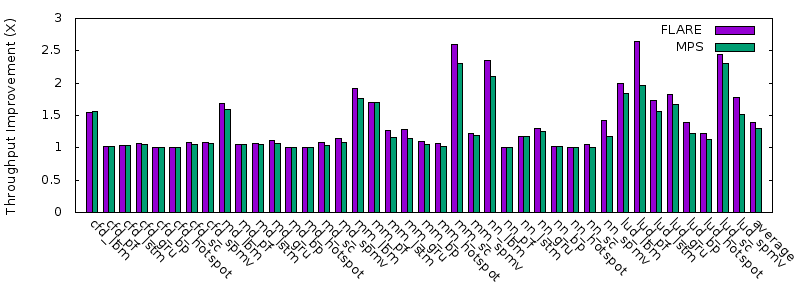
\includegraphics[width=\textwidth, height=2.5cm]{figures/thrpt_res_15.png}
        %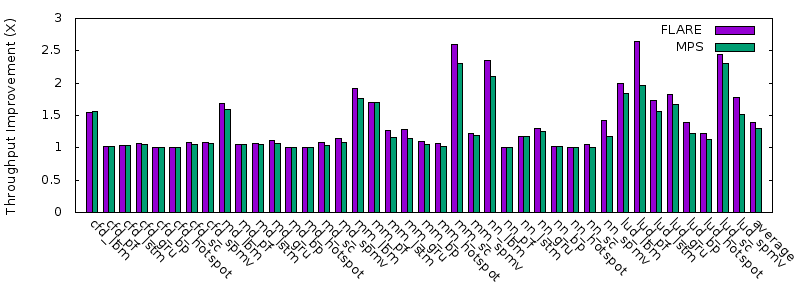
\includegraphics[width=\textwidth]{figures/thrpt_res_15.png}
    %    %\vspace{-0.5cm}
        \caption{Throughput Improvement at 1.5X QoS}
        \label{fig:throughput-results}
        \vspace{-0.5cm}
    \end{figure*}\\
    %\vspace{-1.5cm}
    %\begin{figure*}
    %    \centering
    %    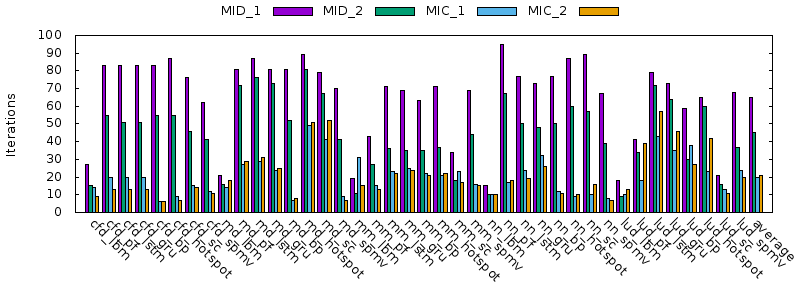
\includegraphics[width=\textwidth, height=2.5cm]{figures/oh_res_12.png}
    %    %\vspace{-0.5cm}
    %    \caption{Online searching overhead at 1.2X QoS}
    %    \label{fig:overhead-results}
        %\vspace{-1cm}
    %\end{figure*}
	%\begin{figure*}
	%	\centering
	%	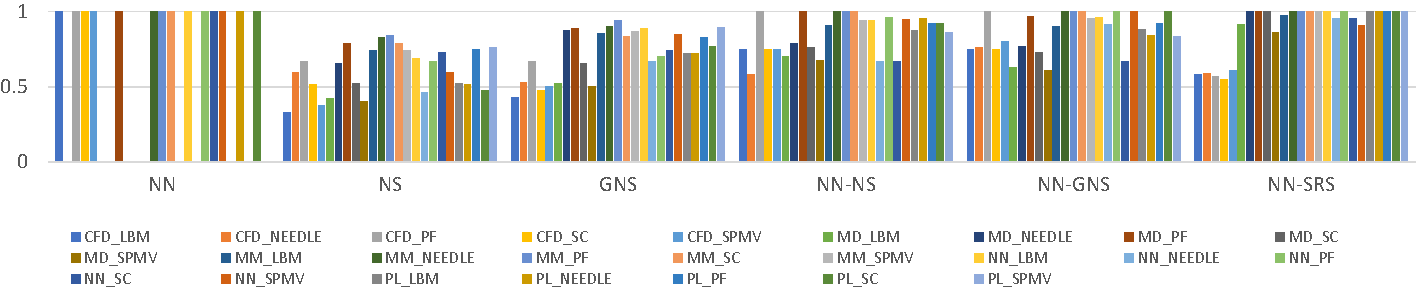
\includegraphics[width=\textwidth]{figures/config_qos_hits_cropped.pdf}
	%	\caption{QoS satisfaction rates of the explored configurations during search.}
	%	\label{fig:config-qos-rate}
	%	%\vspace{-0.5cm}
	%\end{figure*}
%Although the final chosen configuration satisfies QoS as long as dynamic searching is adopted,
%the QoS may be violated during the search process. 
%We observe that the hybrid approaches satisfy QoS more frequently than
%the dynamic only approaches because NN chooses a ``good'' initial configuration and avoids the exploration of configurations
%far from the optimal one.
%\nsout{Figure~\ref{fig:config-qos-rate} shows the fraction of
%iterations which satisfy QoS, where the remainder violate QoS due to choosing detrimental configurations.
%\vspace{1cm}
%\textbf{NN} only explores one configuration, so it either satisfies the QoS %(the bar is of height 1) 
%or misses it. %target, 
%We find that 19 out of 40 co-runs violate QoS in \textbf{NN}. %,
%which makes the NN-only approach unacceptable. %Although the final chosen configuration satisfies QoS as long as dynamic searching is adopted,
%the QoS may be violated during the search process. We observe that the hybrid approaches satisfy QoS more frequently than
%the dynamic only approaches because NN chooses a ``good'' initial configuration and avoids the exploration of configurations
%far from the optimal one.  \\

    \begin{figure*}
    \vspace{-0.5cm}
        \centering
        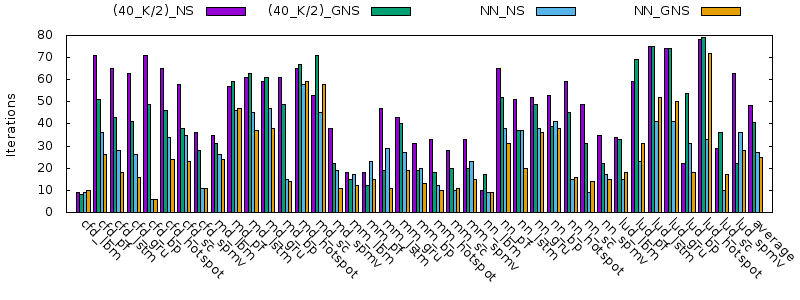
\includegraphics[width=\textwidth, height=2.5cm]{figures/oh_res_15.png}
        %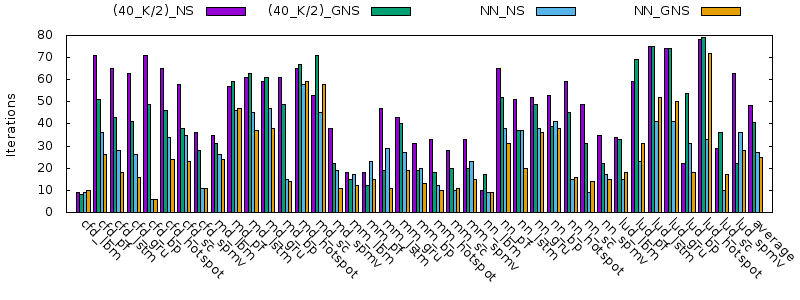
\includegraphics[width=\textwidth]{figures/oh_res_15.png}
        %\vspace{-0.5cm}
        \caption{Online searching overhead at 1.5X QoS}
        \label{fig:overhead-results}
        \vspace{-0.6cm}
    \end{figure*}\\
	%\begin{figure*}%3 out 40 case.\\%and 1 out 40 cases for QoS as 1.2 and 1.5 times of solo-run.
 %The results demonstrate the benefits from spatial
%co-runs enabled by FLARE, which is a key distinction from previous systems.\\
%\subsection{Micro-benchmark Based Performance Degradation Prediction}
\textbf{\textit{Micro-benchmark Prediction Error:}}
%\vspace{-0.5cm}
Fig.~\ref{fig:error} shows the relative error of the performance degradation of LC applications and the relative error of overall throughput predicted
by the \textbf{NN} method for each of the BE and LC kernels. % when QoS is set as 1.2X LC solo-run time. 
%TT and LC in the figure stands for the predictions of overall throughput and latency. %Given the performance degradation of an application as $D$ 
%and the predicted performance degradation due to a co-run as $D'$, 
The relative error is
defined as $|D'-D|/max(D, D')$. The results demonstrate the inefficiency of %the challenge of relying on
model-based approaches to predict performance degradation. For NN\_PF, the prediction
error for %overall 
throughput %of MD\_PF 
and the LC degradation is 
89\% and 92\%, respectively. 
 They are  39\% and 18\% for MM\_PF. The reason is that the applications have
dramatically different properties, such as memory access pattern and branch divergence,
which are difficult to accurately characterize using microbenchmarks. Fortunately, the 
microbenchmarks still capture important features relevant to co-running for a number of
benchmarks. For instance, the prediction errors are as low as 3\% (overall throughput) and 1\% (LC latency) for
CFD\_BP. % co-run. 
On average, the \textbf{NN} method produces 37\% prediction error for the %overall 
throughput and 51\% error for LC latency. % of LC applications. 
Therefore, it is reasonable to use the 
\textbf{NN} method to choose an initial configuration for online search. %Since NN approach does a better job than linear regression
%we do not present detailed data for the linear regression method, which produces much larger (about $2X$ to $5X$) 
%error than nearest neighbor method. 
The NN\_PF pair is an exception in all the pairs. %PF does not like to pair with NN. %If PF co-runs with NN, its performance get hurt significantly. 
No matter how the resources are allocated to PF, the degradation is 15X,
which is why the prediction errors %
%and throughput 
are so large.\\%\vspace{-0.3cm}
    %\begin{figure*}
    %    \centering
    %    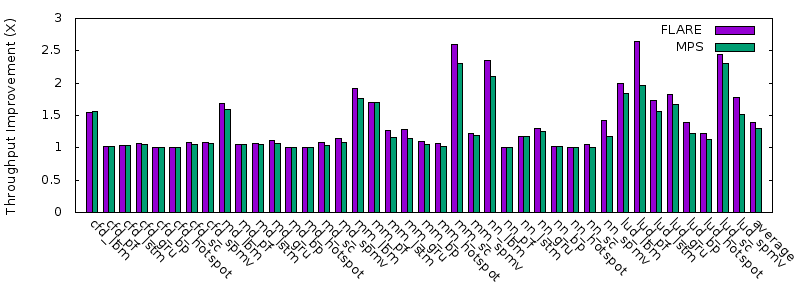
\includegraphics[width=\textwidth,height=2.5cm]{figures/thrpt_res_15.png}
        %\vspace{-0.5cm}
    %    \caption{Throughput Improvement at 1.5X QoS}
    %    \label{fig:throughput-results-1}
        %\vspace{-1cm}
    %\end{figure*}
    %\vspace{-1cm}
    %\begin{figure*}
    %    \centering
    %    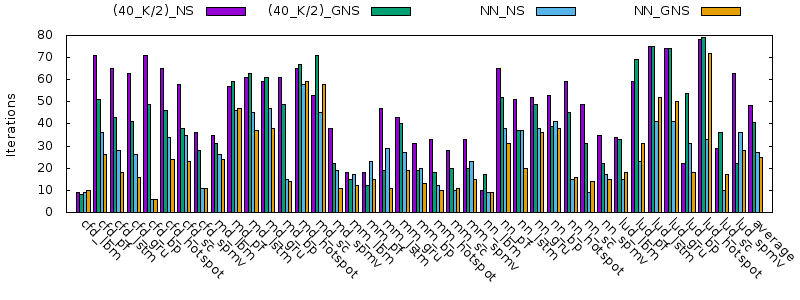
\includegraphics[width=\textwidth, height=2.5cm]{figures/oh_res_15.png}
        %\vspace{-0.5cm}
    %    \caption{Online Searching Overhead at 1.5X QoS}
    %    \label{fig:overhead-results-1}
        %\vspace{-1cm}
    %\end{figure*}
%\subsection{Results on Real Applications}
\textbf{\textit{Real Applications:}}
%\begin{figure}
%		\centering
%		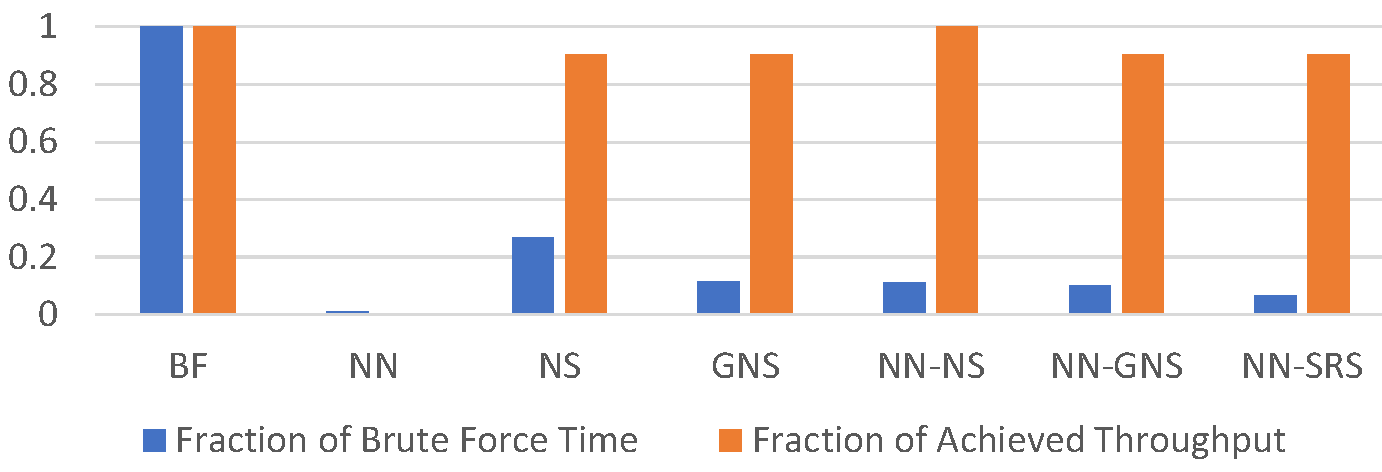
\includegraphics[width=8cm]{figures/real_config_results_cropped.pdf}
%		%\vspace{-0.5cm}
%		\caption{Achieved throughput and runtime overhead when running real applications.}
%		\label{fig:real-config-results}
%	\end{figure}
	%\begin{figure}
	%	\centering
	%	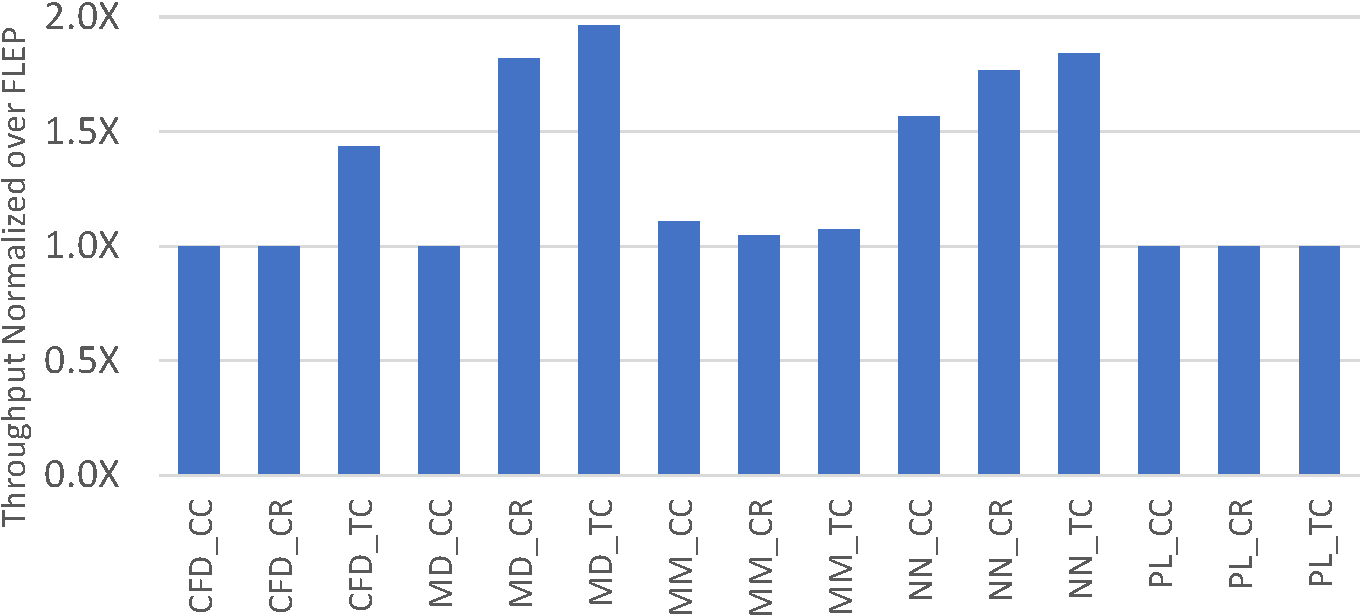
\includegraphics[width=8cm]{figures/real_advantage_cropped.pdf}
	%	\caption{Improvement on hardware utilization when running real applications.}
	%	%\vspace{-0.5cm}
	%	\label{fig:real-advantage}
	%\end{figure}
%We run the two real-world applications (LSTM and GRU) as LC applications paired with 5 benchmarks as BE applications in FLARE.
Fig.~\ref{fig:throughput-results} %and \ref{fig:throughput-results-1} 
show the average throughput improvement across all the co-run pairs including real-world applications for different approaches.
%choosing the co-run configuration that satisfies QoS target.%two objectives of interest at two different QoS target. 
Fig. \ref{fig:overhead-results} %and \ref{fig:overhead-results-1} 
illustrates overheads to
find resource configurations for real-world applications. The pair enclosed in parentheses indicates the initial configuration where $MK$ is the number of maximum thread blocks an SM can host. Similar to the results on benchmarks, \textbf{NN} incurs minimum overhead. \textbf{NN} and \textbf{GNS} %the pure
%dynamic approaches 
need a long search process evidenced by the substantial runtime overhead.
\textbf{NN}, unfortunately, cannot find any configuration that satisfy QoS and hence results from the \textbf{NN} method are not included in these figures.
Dynamic searching algorithms %NN\_NS 
achieve the optimal overall throughput in all the 10 cases. % for two QoS targets.
The average throughput improvement of LSTM and GRU for 5 different pairs is 26\% and 32\%, respectively. %, at 1.2X QoS and they are 46\% and 28\%, respectively for 1.5X QoS.
%The tables \ref{tab:ro-12} and \ref{tab:ro-15} show the overheads of LSTM and GRU pairs at two QoS targets for 4 different approaches. 
The microbenchmark-based methods outperform \textbf{NN} and \textbf{GNS}. %the searches starting at initial guess at (40, 4). 
The overheads with microbenchmark guidance are about 60\% of \textbf{NN} and \textbf{GNS}.% at 1.2 QoS. 
%The former spend about $2/3$ of the time of guess (40, 4) for 1.5 QoS on dynamical searches for the best configuration. 
%\begin{table}
%\begin{minipage}{0.5\linewidth}
    %\centering
%    \begin{tabularx}{\linewidth}{c c c c c}
%    \hline \hline
%         Pair & NN\_NS\_MID & NN\_GNS\_MID & NN\_NS\_MIC & NN\_GNS_MIC \\ \hline
%         LSTM &  79 & 57 & 24 & 28 \\
%         GRU  &  76 & 54 & 27 & 23 \\ 
%         \hline
%    \end{tabularx}
%    \caption{Real-world Pairs Overhead at 1.2X QoS}
%    \label{tab:ro-12}

%\end{minipage}
%\hfill
%\begin{minipage}{0.5\linewidth}
    %\centering
%    \begin{tabularx}{\linewidth}{c c c c c}
%    \hline \hline
%         Pair & NN\_NS\_MID & NN\_GNS\_MID & NN\_NS\_MIC & NN\_GNS_MIC \\ \hline
%         LSTM &  59 & 47 & 44 & 33 \\
%         GRU  &  58 & 51 & 43 & 34 \\ 
%         \hline
%    \end{tabularx}
%    \caption{Real-world Pairs Overhead at 1.5X QoS}
%    \label{tab:ro-15}
%\end{minipage}
%\end{table}
%The overheads of LSTM pairs for 4 approaches (NN\_MID\_1,NN\_MID\_2, NN\_MIC\_1 and NN\_MIC\_2) are 79, 57, 24, and 28 at 1.2X QoS. They are 76, 54, 27, and 23 for GRU pairs.
%At 1.5X QoS, average LSTM and GRU overheads are 
